\documentclass[tikz]{scrartcl}
\usepackage{tikz}
\newcommand{\<}{\textless}
\renewcommand{\>}{\textgreater}
\usetikzlibrary{calc,positioning, shapes, petri, automata,spy}
\tikzset{
    transV/.style={transition, fill=black,font=\footnotesize, minimum height = 12mm, minimum width = 1.5mm,inner sep = 0mm},
    transH/.style={transition, fill=black,font=\footnotesize, minimum width = 12mm, minimum height = 1.5mm,inner sep = 0mm},
    node distance=1.5
}
\usepackage{amsmath,amssymb,amsthm,mathrsfs,amsfonts}

\usepackage{csquotes}
\usepackage{booktabs}

\usepackage{graphicx}
\graphicspath{ {../img/} }
\usepackage{pgfplots}
    \pgfplotsset{
        table/search path={../performance/measurements},
    }

\newcommand{\LSset}[2]{\scriptsize $\begin{aligned}&\{#1\}_L\\&\{#2\}_S\end{aligned}$}



\begin{document}
\begin{tikzpicture}
	\node at (0,0) {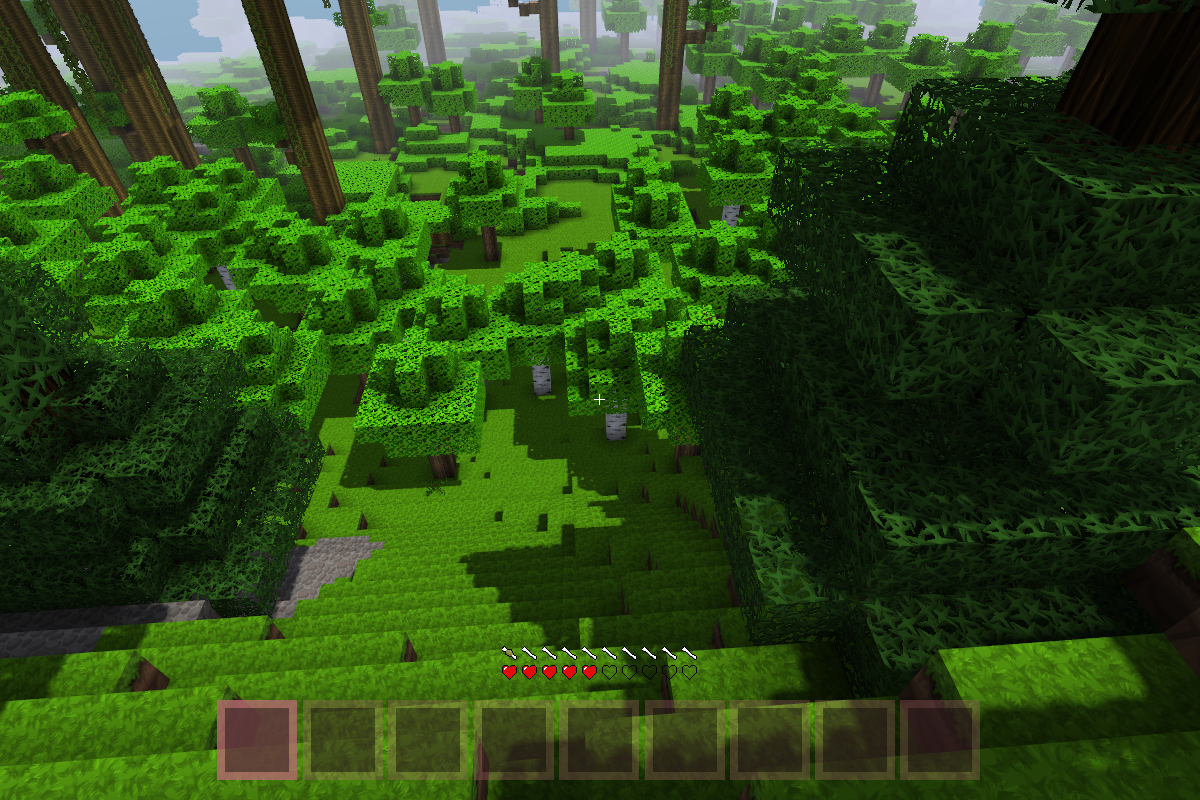
\includegraphics[width=.32\textwidth]{flackern-1.png}};
	\node[draw=red, circle, minimum size = 1.5cm] at (.25,-.5) {};
\end{tikzpicture}

\end{document}